\subsection{Introduction}

The first part of this project was focused on producing a library of autoinducer-antibiotic conjugates. \textit{P. aeruginosa} autoinducers were used, in particular C$_4$-HSL \compound{cmpd:HL4}, HHQ \compound{cmpd:HHQ} and PQS \compound{cmpd:PQS} (see \ref{fgr:PA_autoinducers}). Azido derivatives of these compounds were coupled to alkynyl dervitatives of antibiotics, specifically ciprofloxacin \compound{cmpd:Cip} and trimethoprim \compound{cmpd:Tri} (see \ref{fgr:ABs}), using a copper(I)-catalysed azide-alkyne cycloaddition\cite{Tornoe2002,ANIE:ANIE2596}.

\subsubsection{Azido autoinducer derivatives}

The structure-activity relationships in HHQ \compound{cmpd:HHQ} and PQS \compound{cmpd:PQS} have been previously studied \cite{Lu2012,Lu2014,Hodgkinson2010}, and it was shown various substitutions on the benzene ring could be made without significantly decreasing activity. The 6-azido derivatives (see \ref{fgr:azHHQPQS}) were chosen for this study as routes to them have previously been found\cite{Baker2015}.

%\begin{figure}[H]
%	\begin{center}
%		\schemeref[PQS]{cmpd:PQS}
%		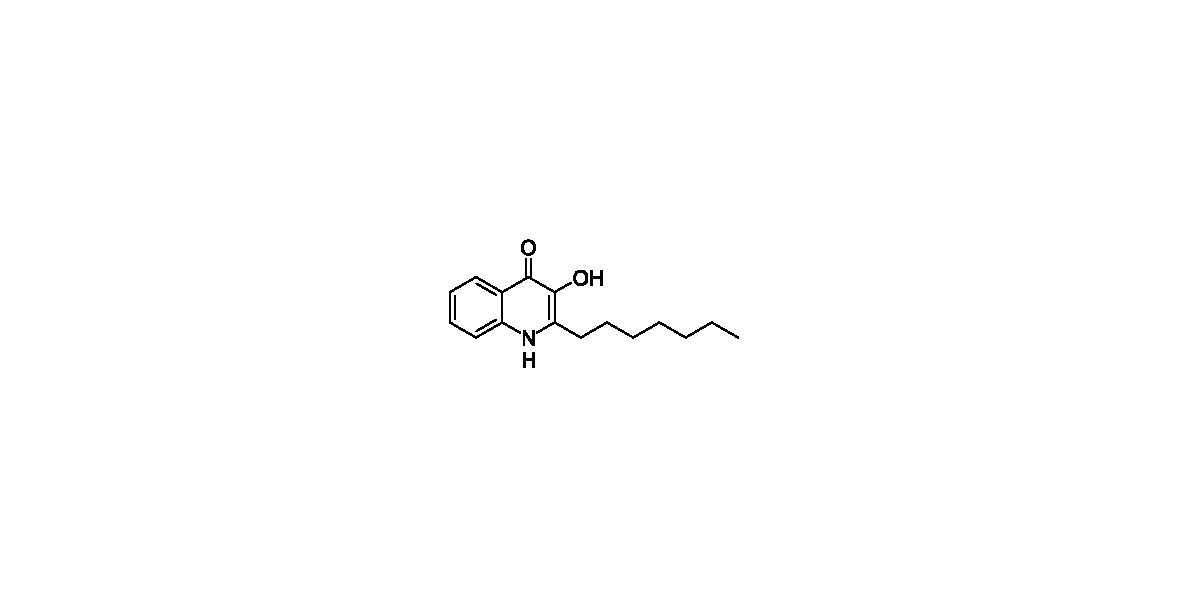
\includegraphics[scale=1]{PQS_num}
%		\caption{The atom numbering in PQS \compound{cmpd:PQS}. \label{fgr:PQS_num}}
%	\end{center}
%\end{figure}

\begin{figure}[H]
	\begin{center}
		\schemeref[azHHQ]{cmpd:azHHQ}
		\schemeref[azPQS]{cmpd:azPQS}
		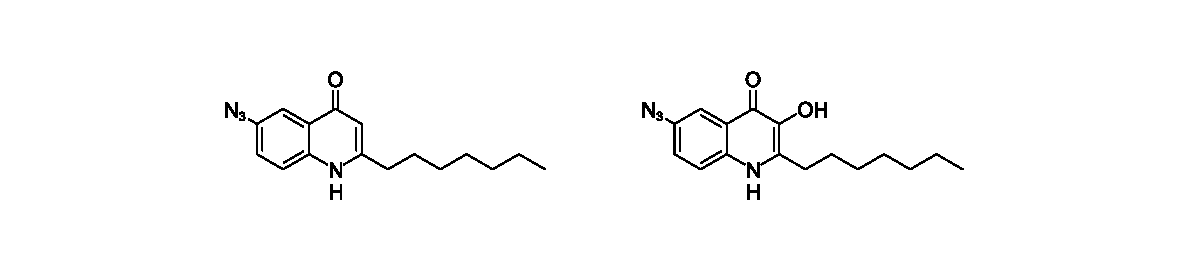
\includegraphics[scale=1]{azHHQPQS}
		\caption{The azido derivatives of HHQ \compound{cmpd:HHQ} and PQS \compound{cmpd:PQS}: \compound{cmpd:azHHQ} and \compound{cmpd:azPQS}. \label{fgr:azHHQPQS}}
	\end{center}
\end{figure}

Alteration of the lactone group of HSL derivatives is known to significantly decrease activity, especially where the number of H-bond donors or acceptors is altered \cite{Galloway2011}. Hence, the azide group was included on the tail\cite{Stacy2013}. Acyl tail length is known to play an important role in affinity\cite{Galloway2011}, so three derivatives of C$_4$-HSL \compound{cmpd:HL4} were synthesised: N$_3$-C$_2$-HSL \compound{cmpd:HL2N3}, N$_3$-C$_4$-HSL \compound{cmpd:HL4N3} and N$_3$-C$_6$-HSL \compound{cmpd:HL6N3} (see \ref{fig:HL_anas}).

\begin{figure}[H]
	\begin{center}
		\schemeref[HL2N3]{cmpd:HL2N3}
		\schemeref[HL4N3]{cmpd:HL4N3}
		\schemeref[HL6N3]{cmpd:HL6N3}
		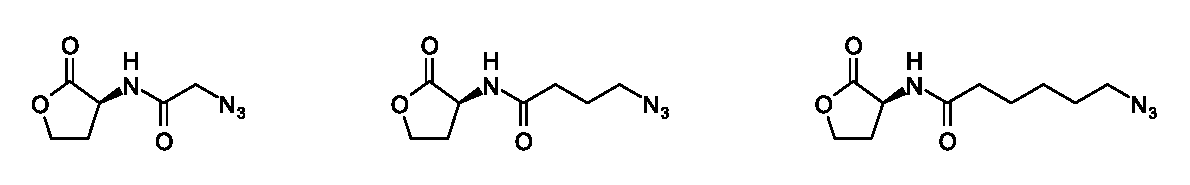
\includegraphics[scale=1]{HL_anas}
		\caption{The azido derivatives of C$_4$-HSL \compound{cmpd:HL4}:  \compound{cmpd:HL2N3}, \compound{cmpd:HL4N3} and \compound{cmpd:HL6N3}. \label{fig:HL_anas}}
	\end{center}
\end{figure}


\subsubsection{Alkynyl antibiotic derivatives}


The structure-activity relationships for ciprofloxacin have been investigated \cite{Renau1996} and modifications at the cyclopropane and piperazine groups were found not to cause loss of activity. It was decided an alkyne tail would be added onto the free NH of the piperazine ring, as this position is more synthetically accessible. Alkynyl ciprofloxacin derivative \compound{cmpd:Y4Cip} (see \ref{fgr:Cip_anas}) was synthesised in this study (see \ref{sec:Y4Cip}), and two cleavable alkynyl ciprofloxacin derivatives \compound{cmpd:Y4HCip} and \compound{cmpd:Y4MeCip} were synthesised by Dr Eddy Sotelo and combined with some of the azido HSL derivatives made in this study (see \ref{sec:HSLs} and \ref{sec:cleavable}).

%\begin{figure}[H]
%	\begin{center}
%		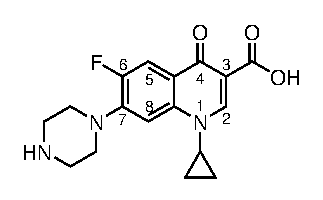
\includegraphics[scale=1]{Cip_num}
%		\caption{The atom numbering in ciprofloxacin \compound{cmpd:Cip}. \label{fgr:Cip_num}}
%	\end{center}
%\end{figure}

\begin{figure}[H]
	\begin{center}
		\schemeref[Y4Cip]{cmpd:Y4Cip}
		\schemeref[Y4HCip]{cmpd:Y4HCip}
		\schemeref[Y4MeCip]{cmpd:Y4MeCip}
		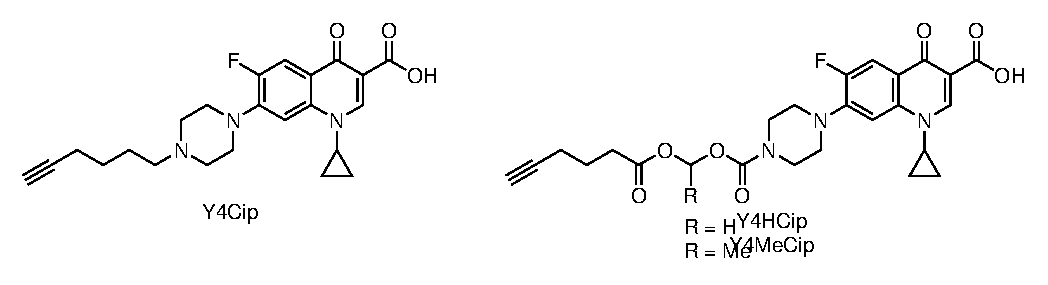
\includegraphics[scale=1]{Cip_anas}
		\caption{The alkynyl ciprofloxacin derivatives \compound{cmpd:Y4Cip}, \compound{cmpd:Y4HCip} and \compound{cmpd:Y4MeCip}. \label{fgr:Cip_anas}}
	\end{center}
\end{figure}



The choice to of alkyne tail attachment point on trimethoprin \compound{cmpd:Tri} (see \ref{fgr:Y4Tri}) is based on the use of that same point in a fluorogenic trimethoprim tag synthesised by Jing \textit{et al}\cite{Jing2013}.

\begin{figure}[H]
	\begin{center}
		\schemeref[Y4Tri]{cmpd:Y4Tri}
		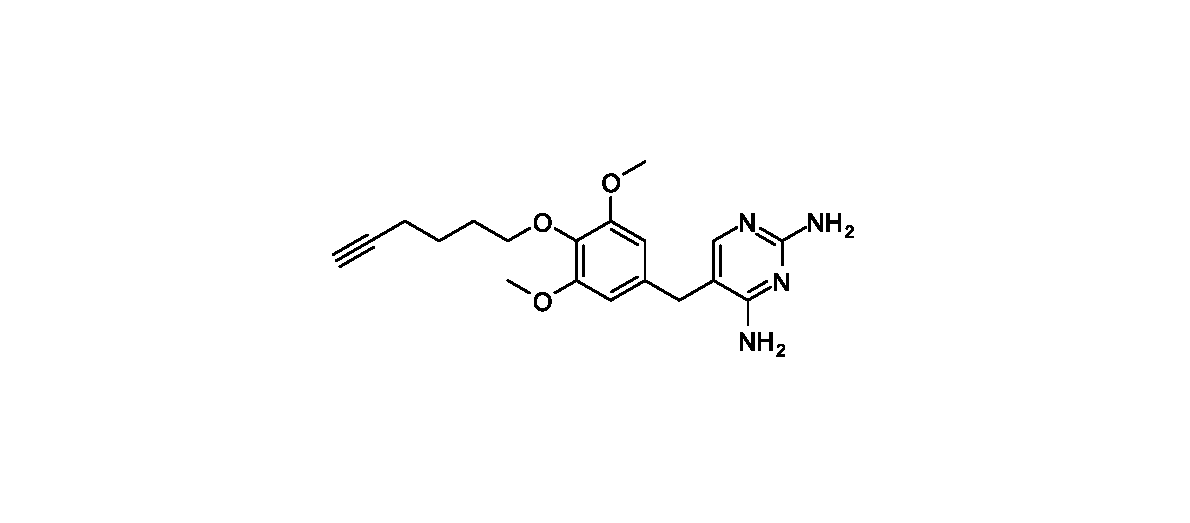
\includegraphics[scale=1]{Y4Tri}
		\caption{The alkynyl trimethoprim derivative \compound{cmpd:Y4Tri}. \label{fgr:Y4Tri}}
	\end{center}
\end{figure}

